% I2C first byte diagram
% Author: Uli Koehler (https://techoverflow.net)
\documentclass[tikz, border=1mm]{standalone}
\usetikzlibrary{positioning, decorations.pathreplacing, arrows.meta}

% Source: https://tex.stackexchange.com/a/24133/45450
\makeatletter
\newcommand*{\textoverline}[1]{$\overline{\hbox{#1}}\m@th$}
\makeatother

\begin{document}
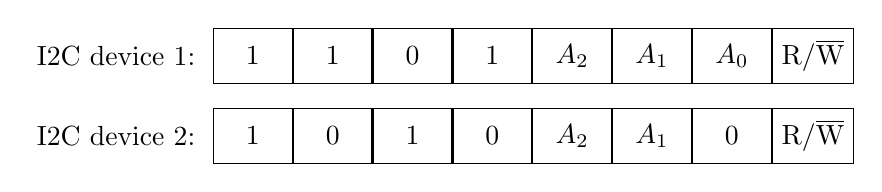
\begin{tikzpicture}
\node (L1) [minimum height=7mm, minimum width=10mm] {I2C device $1$:};
\node (A6) [draw, minimum height=7mm, minimum width=10mm, right=1mm of L1] {1};
\node (A5) [draw, minimum height=7mm, minimum width=10mm, right=0cm of A6] {1};
\node (A4) [draw, minimum height=7mm, minimum width=10mm, right=0cm of A5] {0};
\node (A3) [draw, minimum height=7mm, minimum width=10mm, right=0cm of A4] {1};
\node (A2) [draw, minimum height=7mm, minimum width=10mm, right=0cm of A3] {$A_2$};
\node (A1) [draw, minimum height=7mm, minimum width=10mm, right=0cm of A2] {$A_1$};
\node (A0) [draw, minimum height=7mm, minimum width=10mm, right=0cm of A1] {$A_0$};
\node (RW) [draw, minimum height=7mm, minimum width=10mm, right=0cm of A0] {R/\textoverline{W}};

\node (L2) [minimum height=7mm, minimum width=10mm, below=3mm of L1] {I2C device $2$:};
\node (B6) [draw, minimum height=7mm, minimum width=10mm, right=1mm of L2] {1};
\node (B5) [draw, minimum height=7mm, minimum width=10mm, right=0cm of B6] {0};
\node (B4) [draw, minimum height=7mm, minimum width=10mm, right=0cm of B5] {1};
\node (B3) [draw, minimum height=7mm, minimum width=10mm, right=0cm of B4] {0};
\node (B2) [draw, minimum height=7mm, minimum width=10mm, right=0cm of B3] {$A_2$};
\node (B1) [draw, minimum height=7mm, minimum width=10mm, right=0cm of B2] {$A_1$};
\node (B0) [draw, minimum height=7mm, minimum width=10mm, right=0cm of B1] {0};
\node (RW) [draw, minimum height=7mm, minimum width=10mm, right=0cm of B0] {R/\textoverline{W}};

\end{tikzpicture}
\end{document}